%!TEX root = ../template.tex
%%%%%%%%%%%%%%%%%%%%%%%%%%%%%%%%%%%%%%%%%%%%%%%%%%%%%%%%%%%%%%%%%%%%
%% chapter3.tex
%% NOVA thesis document file
%%
%% Chapter with a short laext tutorial and examples
%%%%%%%%%%%%%%%%%%%%%%%%%%%%%%%%%%%%%%%%%%%%%%%%%%%%%%%%%%%%%%%%%%%%
\chapter{Proposed Solution}
\label{cha:proposed_solution}
After the problem contextualization, and the description of the related concepts, techniques, and studies, this chapter presents the work already prepared. Starting with the requirements analysis which includes user interviews and extraction of metrics to conclude, in quantitative manners, what type of cases could lead to \gls{SQL} usage. A current progress state of the solution developed will be presented, describing the actual development state and a foreseeing schedule of the work plan for the remaining time until the final of the dissertation.

\section{Requirements Analysis}
\label{sec:requirements_analysis}
In order to understand the functionalities and visual approaches used by Aggregates to visually build queries, the project has started with an exploration of this system (more detailed description ins section \ref{subsec:visual_data_querying}). Meanwhile, not only were identified the expressiveness problems of the visual language, previously mentioned in section \ref{sec:problem_description}, but also usability problems could be perceived in the performance of available actions. 

After that, user interviews have been prepared to explore the limits of the tool and understand the impact of the problems on user actions. So, in the interviews, after perceiving the background of the participant, more directed questions were asked to pick up the first responses of the users about the advantages and disadvantages of the visual query tool. Next, it was asked what are the situations when \gls{SQL} usage was preferred to obtain insights about the reasons not to use the visual tool to perform these queries. Also, it was required that users present examples to explain the problems they have, whenever possible, because this strategy can be useful to understand the impact level of the problem and sometimes show other problems not primarily identified. In addition, when the users did not mention anything about expressiveness problems of the visual tool, direct questions about if they never needed to use the operations not supported by Aggregates were asked to cover the possibility of forgetting to mention that aspect.

The results reveal that the most novice users, with less than six months of experience, feels that Aggregates are easy to use and covers their necessities, referring also that were simpler to learn than \gls{SQL}. The most experienced users, who use the OutSystems platform to develop applications, every day, for professional purpose, and have a technological background, reported that in the visual tool they cannot have a good understanding of the global view of the query, mainly if many tables, columns and business rules are involved. Switch between tabs in the interface to view the data sources, and the filtering and sorting criteria were other issue presented, as well as the lack of control on the query output \footnote{As referred on section \ref{subsubsec:current_progress}, when a user adds an entity to an Aggregate, all its attributes are added automatically and if the user hides them the output of the query does not change.}. Asked about the aggregation functions \footnote{Funtionality added when Simple Queries have been replaced by Aggregates (Section \ref{subsubsec:previous_work})}, they do not refer any problem with the approach interaction strategy adopted. Furthermore, other usability problems that decrease the users’ satisfaction have been pointed out, like the difficulty to search for a column in the query result, when there are numerous columns.

The analysis was complemented with a metric study on queries executed on the Outsystems cloud, in order to find patterns that could justify users reasons to use \gls{SQL} instead of Aggregates. The queries analysed, which have been extracted in July 2019 from customers’ projects, were built using Advanced Queries \footnote{The option of the OutSystems Platform, invoked in section \ref{subsubsec:previous_work}, that allows the query design in a textual way using a language based on \gls{SQL}.}.

Firstly, the data set is composed of 214.400 statements, but only 60.8\% were used in this study since only the queries were important for this context and not other instructions, such as inserts, updates, deletes, and transactions. Since the last set, which includes 125.613 queries, has duplicated queries, these were removed and the final queries set used to extract information comprehends 67.828 queries. The operators and clauses were figured out using a \gls{SQL} Parser developed in JavaScript \footnote{js-SQL-parser repository page: \url{https://github.com/JavaScriptor/js-SQL-parser}}.

After the abstract syntax trees of the queries were obtained in a JSON file, these were analysed in a program to count the operators and the clauses that were present in the queries. A first analysis can measure the operators that are not supported by the visual tool, since the textual language is the only way to perform these operations. Table \ref{tab:aggregates_operations_not_supported_stats} summarizes the number of queries that contain these operations, where the intersection is not null, so there are queries that have two or more of the indicated operations. Thus, each percentage represents the subset of queries that use the operation inside, no matter if they have other operations or not.

%\begin{figure}[htbp]
%	\centering
%	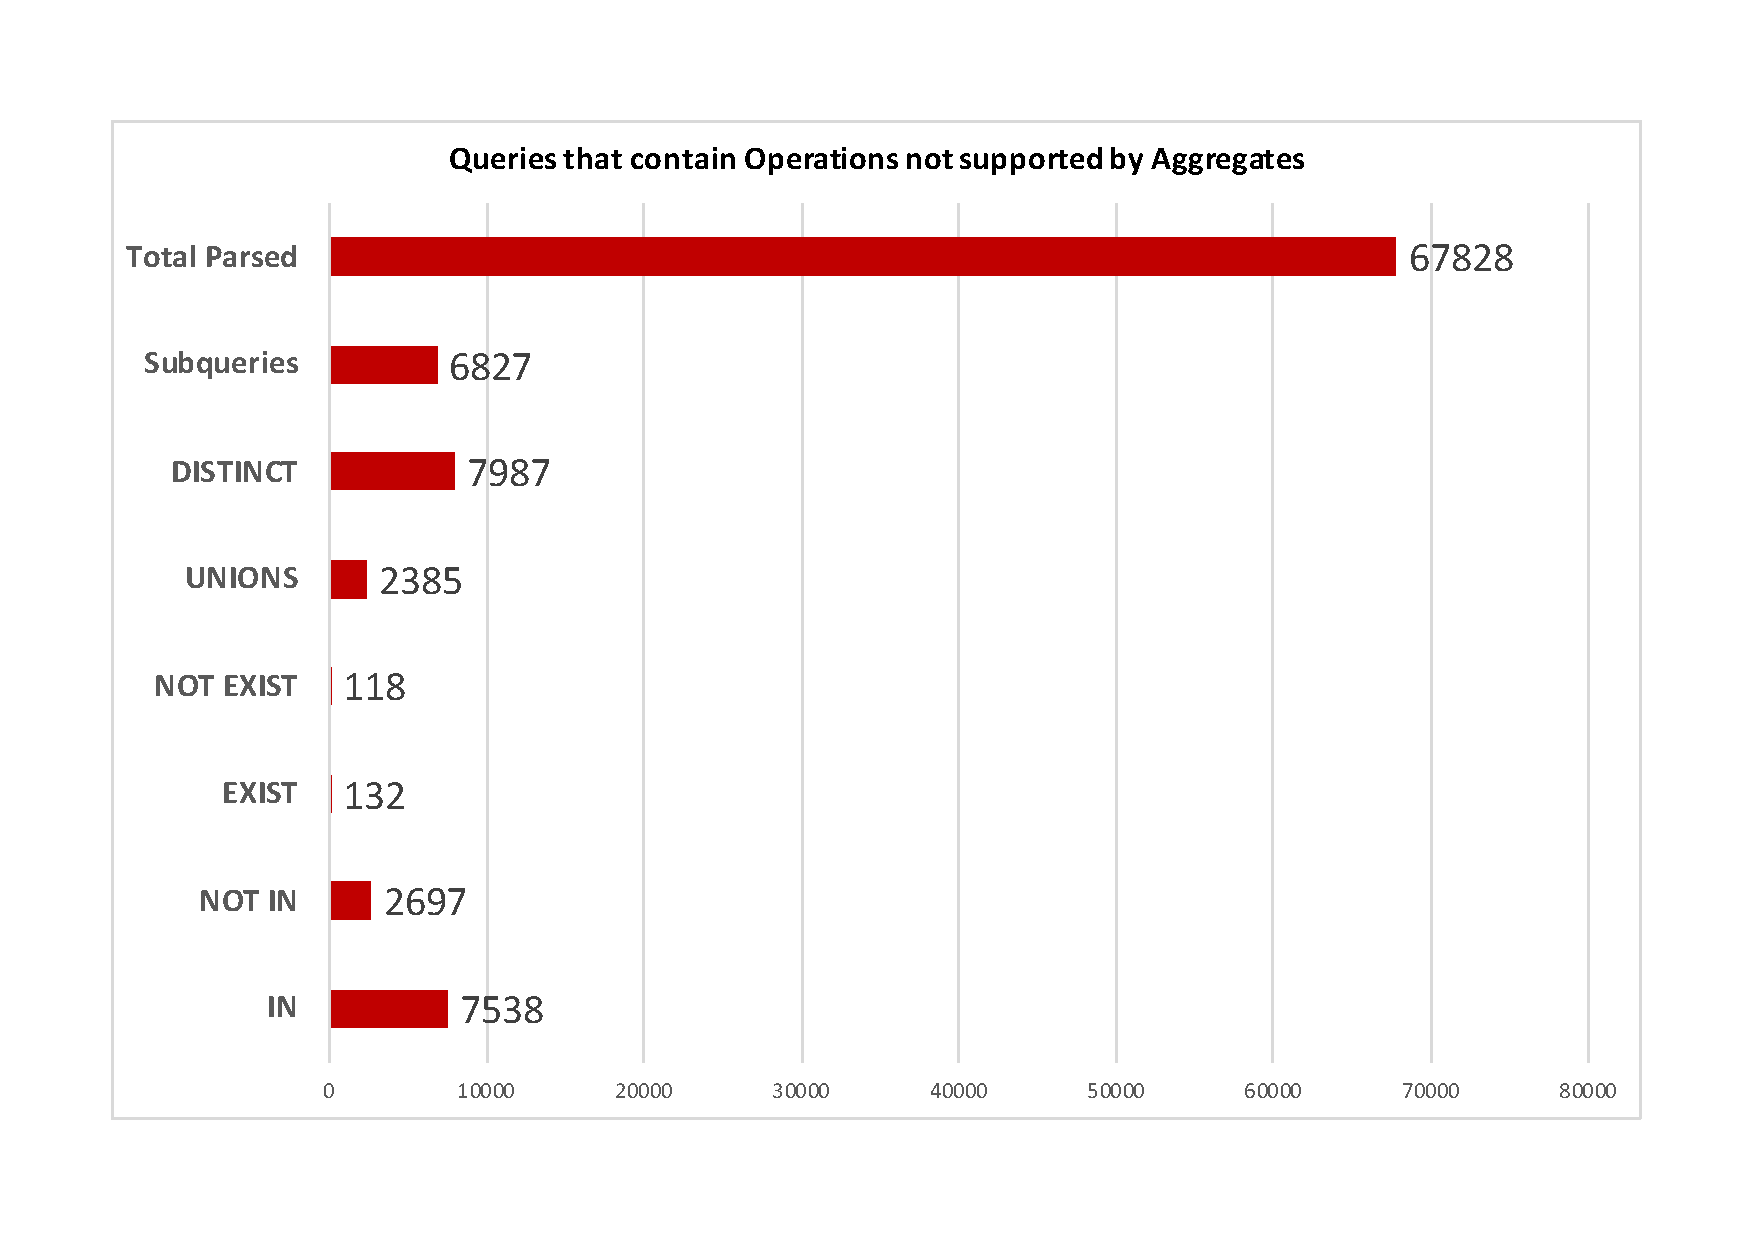
\includegraphics[height=3in]{ChartOperationsNotSupported}
%	\caption{Number of the queries that contain operations not supported by Aggregates}
%	\label{fig:aggregates_operations_not_supported_stats}
%\end{figure}

\begin{table}[tb]
	\caption{Queries that contain operations not supported by Aggregates}
	\label{tab:aggregates_operations_not_supported_stats}
\centering
\resizebox{\textwidth}{!}{
\begin{tabular}{c|c|c|c|c|c|c|c|c|}
    \cline{2-9}
    \rowcolor[HTML]{C0C0C0} 
    \cellcolor[HTML]{FFFFFF}                                 & IN      & NOT IN & EXIST  & NOT EXIST & UNIONS & DISTINCT & SUBQUERIES & Total \\ \hline
    \multicolumn{1}{|c|}{\cellcolor[HTML]{C0C0C0}Queries}    & 7538    & 2697   & 132    & 118       & 2385   & 7987     & 6827       & 67828 \\ \hline
    \multicolumn{1}{|c|}{\cellcolor[HTML]{C0C0C0}Percentage} & 11.11\% & 3.98\% & 0.19\% & 0.17\%    & 3.52\% & 11.78\%  & 10.07\%    & 100\% \\ \hline
    \end{tabular}
}
\end{table}

Furthermore, it was measured how many queries are performed using the textual language but could be designed using Aggregates. Table \ref{tab:aggregates_supported_vs_not_supported_stats} shows the results obtained that divide the queries performed in three categories:

\begin{itemize}
    \item Not Supported: Queries which include operations not supported by Aggregates, such as IN, NOT IN, EXIST, NOT EXIST, Unions, Distincts and Subqueries;
    \item Supported by Aggregates: Queries that could be designed totally using Aggregates. These are divided into two subcategories:
    \begin{itemize}
        \item Simpler: Queries which include only operations supported by aggregates excluding the indication of sorting criteria and the use of aggregation functions (e.g. GROUP BY or SUM, AVG, MIN, MAX, COUNT);
        \item More Complex: Queries that are supported by Aggregates excluding the above (simplers).
    \end{itemize}
\end{itemize}

Since user interviews suggested that aggregation functions and sorting criteria were not the main problems. The queries supported by Aggregates were divided to compare the quantitative analysis with the qualitative analysis extracted in interviews. This is important because these operations can be specified using a different interaction technique where the user changes the query when he is interacting with the query result, as mentioned in section \ref{subsubsec:current_progress}. 

\begin{table}[tb]
	\caption{Queries that could be designed using Aggregates and the queries which the tool does not support}
	\label{tab:aggregates_supported_vs_not_supported_stats}
\centering
\resizebox{\textwidth}{!}{
\begin{tabular}{c|c|c|c|c|}
    \cline{2-5}
    \rowcolor[HTML]{C0C0C0} 
    \cellcolor[HTML]{FFFFFF}                                 & Not Supported & Supported (Simpler) & Supported (More Complex) & Total \\ \hline
    \multicolumn{1}{|c|}{\cellcolor[HTML]{C0C0C0}Queries}    & 28130         & 24026               & 15672                    & 67828 \\ \hline
    \multicolumn{1}{|c|}{\cellcolor[HTML]{C0C0C0}Percentage} & 41.5\%        & 35.4\%              & 23.1\%                   & 100\% \\ \hline
    \end{tabular}
    }
\end{table}


\section{Scope Definition}
\label{sec:scope_definition}
The results of the quantitative analysis show that it is in conformity with the qualitative analysis results (user interviews). Both of the analysis, concludes that the main priority of the project should be the usability improvement of the visual querying tool interface. 
%since not only is the main concerned pointed out by the users, but also has metrics that sustain that hypothesis. 
In the set of queries analysed, around 58.5\% could be designed using Aggregates, is evident that the lack of support of some \gls{SQL} expressions might not be the main problem.

Although the results show a small set of queries that are not supported, these expressiveness problems of the visual tool can influence users to change to the textual languages. So, as the visual approach does not support some features users may want to change to the textual language where they can perform all the queries.

Under the circumstances, the results were discussed together with the stakeholders. It was determined that the main problem was the usability of the system. Regarding the improvement of the visual interface expressiveness, it was defined that the main priorities were the IN / NOT IN and the DISTINCT operations. Thus, along with the project, the main focus will be the improvement of the usability and if it is possible conciliating to these two new features of visual expressiveness.

\section{Proposed Implementation}
\label{sec:proposed_implementation}
According to the analysis made and the results concluded, the implementation covers an iterative design process aiming at improving the usability of Aggregates, the component of the OutSystems Platform to visually build queries. The prioritized improvements of the \gls{VQL} expressiveness (IN / NOT IN and DISTINCT) will be included in the project, if possible, depending on the development progress of the usability issues. If in the next stages of development it is found that it is possible to address these expressiveness problems without impairing the development related to improving usability, these will be designed and developed, otherwise, the focus will be only the usability improvement. %TODO: Falta explicar melhor em que consiste melhorar a usabilidade, resumindo quais sao os problemas

As mentioned above in Section \ref{subsubsec:current_progress}, the actual visual tool include in the interface sections to design queries visually and to view their results. Therefore, the aim is to design and evaluate how these two parts of the interface can be changed to improve the usability of the system. In a nutshell, there are two aspects that are needed to be taken into account, in order to guide the design process: the simplicity, efficiency and effectiveness to construct queries independently of how many tables or conditions, and the readability of the global query to perceive what data of the database the query will be gathering.

%Never forgetting these guidelines, the query parts specified in Table X will guide the design process, studying and evaluating solutions to improve the specification method, without harming the query overview readability and the interaction strategies to specify the other parts of the query. 

The design and development process shall be divided into an initial preparation and analysis phase and the iterative design process phase:

\begin{itemize}
    \item \textbf{Preparation and analysis phase}: before the development of the prototypes, the users and the tasks of the should be analysed. Also, it should be started sketching as a means to bring up ideas that could represent starting points to tackle the existing problems. Therefore, this preparation process before the development of the prototypes will include the following tasks:
    \begin{itemize}
        \item \textbf{Data Extraction}: although there are results obtained in the interviews and in the quantitative analysis process, detailed in \ref{sec:requirements_analysis}, additional data about the queries design using aggregates also will be extracted. It could be important to the process to understand the user's usage of the existing visual tool since the results obtained are only about the queries built using the textual language;
        \item \textbf{User and Task Analysis}: users and their tasks will be characterized and classified regarding the concepts presented in section \ref{subsubsec:user_and_task_analysis} This description and classification will be used not only as a reference point throughout the design process but also to define the most important trade-offs on usability attributes;
        \item \textbf{Sketching}: the phase where the first sketches of possible solutions will be designed. The most important is the initial exploration of several possibilities to tackle the problems through a low-level and fast approach. As referred in section \ref{subsubsec:sketching_and_prototyping} it is useful to discover new ideas, keeping register the first approaches to tackle the problems. At the later phases, the sketches could be useful to remember the starting point of the design process;
    \end{itemize}
    \item \textbf{Iterative design}: this process starts with low-level prototypes and in each iteration, these are evaluated to create higher fidelity prototypes in the next iteration. However, as referred in section \ref{subsubsec:sketching_and_prototyping}, there are different strategies to reuse or not the prototypes over iterations. In this project, an evolutionary strategy where the prototypes developed are used as the basis for the next design iteration will be adopted. Moreover, the design process will include three iterations:
    \begin{itemize}
        \item \textbf{Paper Prototype (1st iteration)}: regarding the information obtained in user and task analysis, and the main ideas raised on the sketching stage, a first functional paper prototype will be built. The evaluation of the entire concept of the first interaction strategies is the main concern of this phase. Cognitive Walkthrough and Observational Methods of user testing will be the evaluation techniques used on this phase;
        \item \textbf{Low-fidelity Prototype (2nd iteration)}: using the results of the previous iteration, the idea is to develop a low-fidelity computer prototype on technologies, such as Balsamiq \cite{balsamiq} or Mockingbird \cite{mockingbird}, which although do not create native applications, allow the employment of visual components and animations more similar with the intended in the final solution. So, more aspects can be tested regarding a higher complexity and fidelity of the interface. At this stage, Heuristic Evaluation will be used by experts and more user tests will be performed. The type of user tests to be made will depend on the results obtained. However, it is likely that not only Observational Methods are performed. Experimental Methods could be necessary to test specific hypotheses or discuss what is the better option between a set of possible implementations. Moreover, Query Methods, like questionnaires, could be valuable as well, to understand the user’s satisfaction;
        \item \textbf{Final Prototype (3rd iteration)}: computer prototype integrated in the OutSystems Platform. The development focuses on the presentation layer of the application due to improving the Aggregates interface and \gls{UX}, using the new results obtained. Being the last prototype and consequently the final result of this project, it will be evaluated also by users and experts to summarize the final results of all the design and development process;
    \end{itemize}

\end{itemize}

\section{Work Plan}
\label{sec:work_plan}
According to the proposed implementation approach, Figure \ref{fig:work_plan} represents a work plan until the final of the thesis, scheduling each one of the tasks explained in the previous section throughout the remaining weeks. The tasks are assigned to its respective major phases, and the focus on the writing of the document is primarily at the end of each phase or iteration to summarize all the contents addressed during these periods, although the report can be updated every time it reveals useful.

\begin{figure}[htbp]
	\centering
	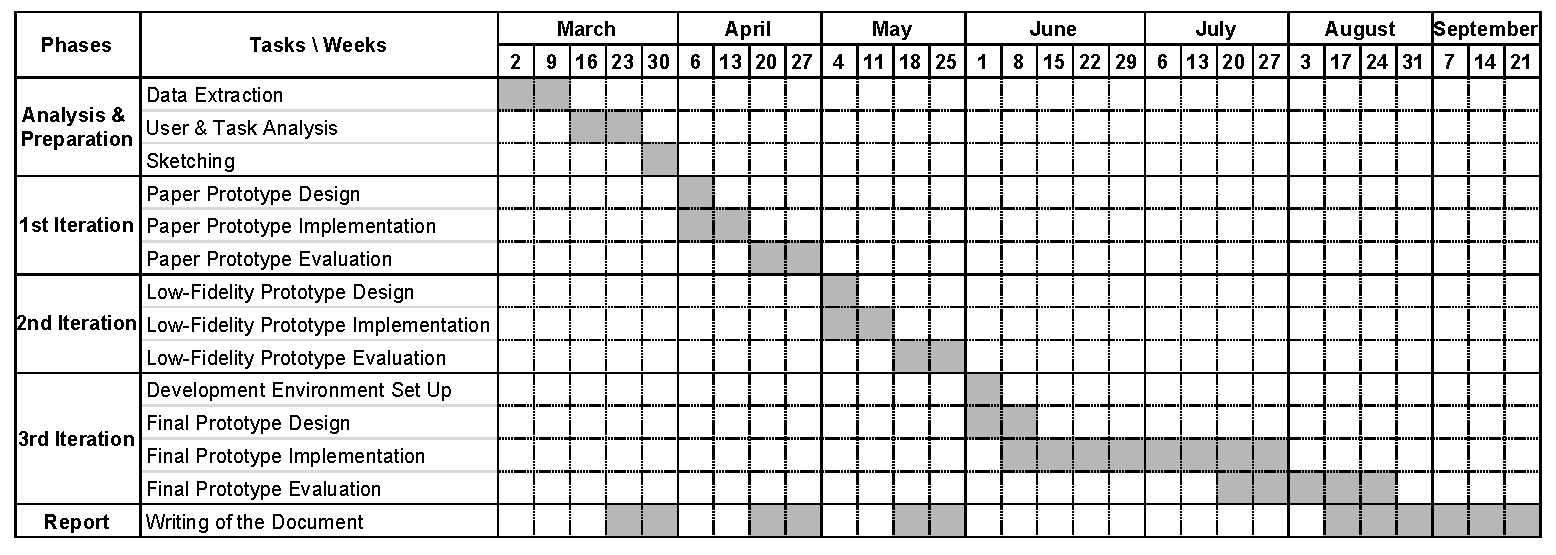
\includegraphics[width=1.0\textwidth]{workPlan}
	\caption{Task Scheduling throughout the weeks until the final of the project.}
	\label{fig:work_plan}
\end{figure}



